\documentclass[a4paper,10pt]{article}
\usepackage[utf8x]{inputenc}
\usepackage[spanish]{babel}
\usepackage{graphicx}
\usepackage{multicol}
\usepackage[right=2cm,left=2cm,top=2cm,bottom=3cm]{geometry}


%opening
\title{B\&B}
\author{andrea}

\begin{document}

\maketitle

\section{Branch and Bound}

Para la variables binarias que dan soporte a las restricciones relacionadas con los valores absolutos de las distancias y la función objetivo y que la ciudad más cercana corresponda
a una ciudad del problema. Para ver mayor información revisar la sección \textbf{Variables Binarias del Problema}.\\

Para el algoritmo \emph{Branch and Bound} (\textbf{B\&B}) usamos la implementación en la librería \emph{LpSolve}. Dicha librería trae varias heurísticas con las cuales usar
el B\&B, además de las heurísticas para elegir la rama a tomar, también esta disponible la opción de si iniciar la rama con la función techo o con la función piso.\\

De las heurísticas que están disponibles en \emph{LpSolve} elegimos 13 para comparar el rendimiento. Además por cada heurística ésta se probó con la función techo y la función piso, para 
evaluar la mejor combinación. A continuación se explica el proceder de las 13 heurísticas\footnote{fuente: http://lpsolve.sourceforge.net/5.5/set\_bb\_rule.htm}:

\begin{enumerate}
 \item \textbf{NODE\_FIRSTSELECT}: Elige la primera columna no entera.%1
 \item \textbf{NODE\_GAPSELECT}: Selecciona la variable de acuerdo a la distancia de los límites actuales.%2
 \item \textbf{NODE\_RANGESELECT}: Selecciona la variable de acuerdo al mayor límite actual.%3
 \item \textbf{NODE\_FRACTIONSELECT}: Selecciona la variable que tenga el valor fraccionario más grande.%4
 \item \textbf{NODE\_PSEUDOCOSTSELECT}: Selecciona la variable con la estrategia pseudo-costo (búsqueda costo uniforme)%5
 \item \textbf{NODE\_PSEUDONONINTSELECT}: Es una extensión de la estrategia pseudo-costo basada en minimizar el número de enteros fallidos.%6
 \item \textbf{NODE\_PSEUDORATIOSELECT}: También es una extensión de la estrategia pseudo-costo basada en maximizar la razón pseudo-cost divido por el número de fallidas. Similar a costo/beneficio.%7
 \item \textbf{NODE\_WEIGHTREVERSEMODE}: Selecciona la variable por el peor criterio en vez del mejor criterio.%8
 \item \textbf{NODE\_GREEDYMODE}: Búsqueda informada, con un costo heurístico.%9
 \item \textbf{NODE\_DEPTHFIRSTMODE}: Búsqueda en profundidad, selecciona el nodo por el que ya venia explorando.%10
 \item \textbf{NODE\_RANDOMIZEMODE}: Añade un factor random al costo de un nodo candidato.%11
 \item \textbf{NODE\_BREADTHFIRSTMODE}: Selecciona el nodo que no se halla seleccionado o que se halla seleccionado menos veces (anteriormente).%12
 \item \textbf{NODE\_AUTOORDER}: Crea una variable de ordenamiento ``óptima'' para el B\&B. (Indexación)%13
\end{enumerate}


Para realizar la pruebas correspondientes se generaron $20$ ejemplos aleatorios. 5 ejemplos con una grilla de tamaño $5$ y número de ciudades aleatorio, 5 ejemplos con una grilla
de tamaño $10$ y número de ciudades aleatorio, 5 ejemplo con una grilla de tamaño $15$ y número de ciudades aleatorio y 5 ejemplos con una grilla de tamaño $20$ y número de ciudades aleatorio.
A cada ejemplo se le aplica el algoritmo con cada heurística una vez con la función techo y otra con la función piso.\\

Comparamos el desempeño de las heurísticas usando la función techo con los 5 ejemplos de un tamaño de grilla y así con todos los tamaños de la grilla. Se comparaban las heurísticas en 3 tres grupos,
por cada grupo se seleccionaba la heurística con el mejor desempeño, y al final se eligió la mejor de las tres mejores. Este fue el procedimiento aplicado para las comparaciones por ejemplos. Finalmente
se realizó una comparación entre todos los ejemplos (se eligió el un ejemplo por cada tamaño de grilla, el que tuviera mas ciudades) para elegir las 3 mejores heurísticas, dichas heurísticas
usaban la función piso. \\

\subsection{Ejemplos tamaño de grilla 5}

Gráficas correspondientes al desempeño de las heurísticas, 3 grupos:\\
\textbf{Usando techo:}


\begin{figure}[ht]
\begin{minipage}[b]{0.45\linewidth}
 \centering
 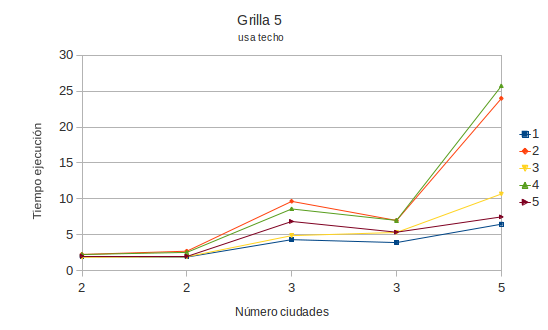
\includegraphics[width=\textwidth]{grilla5ceil0.png}
 % grilla5ceil0.png: 548x330 pixel, 72dpi, 19.33x11.64 cm, bb=0 0 548 330
 \caption{Comparación heurísticas  1 $\cdots$ 5}
 \label{fig:grid5ceil0}
\end{minipage}
\hspace{0.5cm}
\begin{minipage}[b]{0.45\linewidth}
 
\centering
 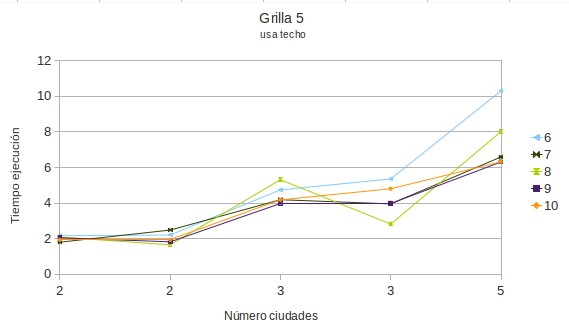
\includegraphics[width=\textwidth]{grilla5ceil1.png}
 % grilla5ceil0.png: 548x330 pixel, 72dpi, 19.33x11.64 cm, bb=0 0 548 330
 \caption{Comparación heurísticas  6 $\cdots$ 10}
 \label{fig:grid5ceil1}
\end{minipage}

\begin{minipage}[b]{1\linewidth}
  \centering
 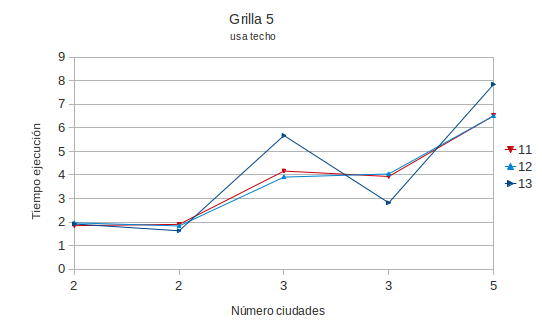
\includegraphics[scale=0.4]{grilla5ceil2.png}
 % grilla5ceil0.png: 548x330 pixel, 72dpi, 19.33x11.64 cm, bb=0 0 548 330
 \caption{Comparación heurísticas  11 $\cdots$ 13}
 \label{fig:grid5ceil2}
\end{minipage}

\end{figure}


De la figura \ref{fig:grid5ceil0} la heurística que presentó mejor desempeño fue la número $1$ (NODE\_FIRSTSELECT), de la figura \ref{fig:grid5ceil1} fue la número $9$ (NODE\_GREEDYMODE) y de la 
figura \ref{fig:grid5ceil2} fue la número $12$ (NODE\_BREADTHFIRSTMODE). Al comparar éstas tres, la mejor correspondió a la heurística número $9$ (NODE\_GREEDYMODE).

\begin{figure}[ht]
\begin{minipage}[b]{1\linewidth}
 \centering
 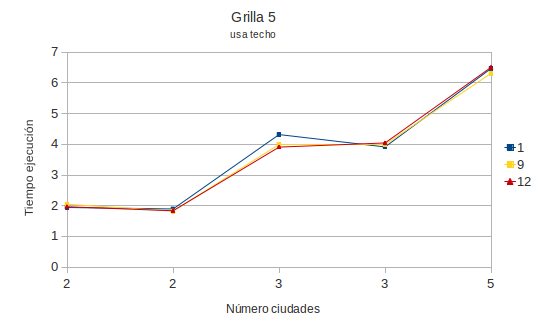
\includegraphics[scale=0.4]{grilla5ceil3.png}
 % grilla5ceil3.png: 539x326 pixel, 72dpi, 19.01x11.50 cm, bb=0 0 539 326
 \caption{Comparación mejor heurística}
 \label{fig:grid5ceil3}
\end{minipage}
\end{figure}

\newpage

\textbf{Usando piso:}

\begin{figure}[ht]

\begin{minipage}[b]{0.45\linewidth}
 \centering
 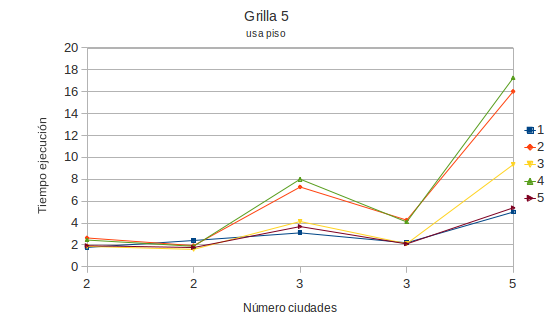
\includegraphics[width=\textwidth]{grilla5floor0.png}
 % grilla5ceil0.png: 548x330 pixel, 72dpi, 19.33x11.64 cm, bb=0 0 548 330
 \caption{Comparación heurísticas  1 $\cdots$ 5}
 \label{fig:grid5floor0}
\end{minipage}
\hspace{0.5cm}
\begin{minipage}[b]{0.45\linewidth}
 \centering
 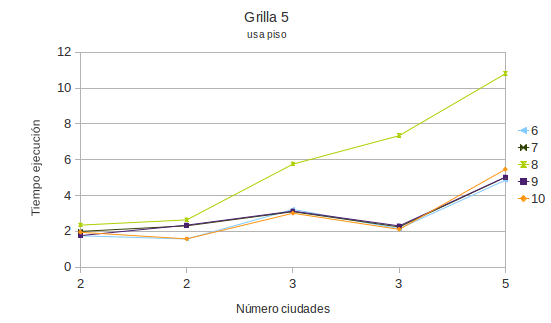
\includegraphics[width=\textwidth]{grilla5floor1.png}
 % grilla5ceil0.png: 548x330 pixel, 72dpi, 19.33x11.64 cm, bb=0 0 548 330
 \caption{Comparación heurísticas  6 $\cdots$ 10}
 \label{fig:grid5floor1}
\end{minipage}

\begin{minipage}[b]{1\linewidth}
  \centering
 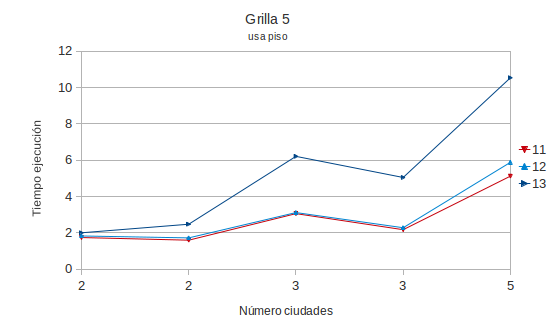
\includegraphics[scale=0.4]{grilla5floor2.png}
 % grilla5ceil0.png: 548x330 pixel, 72dpi, 19.33x11.64 cm, bb=0 0 548 330
 \caption{Comparación heurísticas  11 $\cdots$ 13}
 \label{fig:grid5floor2}
\end{minipage}

\end{figure}


De la figura \ref{fig:grid5floor0} la heurística que presentó mejor desempeño fue la número $1$ (NODE\_FIRSTSELECT), de la figura \ref{fig:grid5floor1} fue la número $6$ (NODE\_PSEUDONONINTSELECT) y de la 
figura \ref{fig:grid5floor2} fue la número $11$ (NODE\_RANDOMIZEMODE). Al comparar éstas tres, la mejor correspondió a la heurística número $6$ (NODE\_PSEUDONONINTSELECT).

\begin{figure}[ht]
\begin{minipage}[b]{1\linewidth}

 \centering
 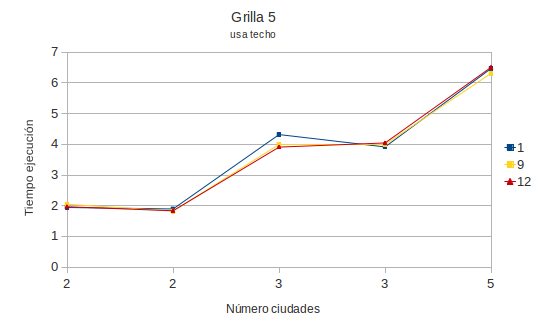
\includegraphics[scale=0.4]{grilla5ceil3.png}
 % grilla5ceil3.png: 539x326 pixel, 72dpi, 19.01x11.50 cm, bb=0 0 539 326
 \caption{Comparación mejor heurística}
 \label{fig:grid5floor3}
\end{minipage}
\end{figure}

\newpage

\textbf{Comparación mejor techo-piso}

Tomamos la mejor heurística usando techo y la mejor heurística usando piso, comparamos sus resultados con los ejemplos y concluimos que la mejor era la número $6$, que usaba piso.

\begin{table}
    \begin{tabular}{|c|c|}
        \hline
        6  \\ PSEUDONONINTSELECT & 9  \\ GREEDY \\ \hline
        1,753                            & 2,05              \\ \hline
        1,573                            & 1,824             \\ \hline
        3,223                            & 3,993             \\ \hline
        2,154                            & 3,998             \\ \hline
        4,858                            & 6,313             \\
        \hline
    \end{tabular}
\end{table}

\begin{figure}[ht]
\begin{minipage}[b]{1\linewidth}
 \centering
 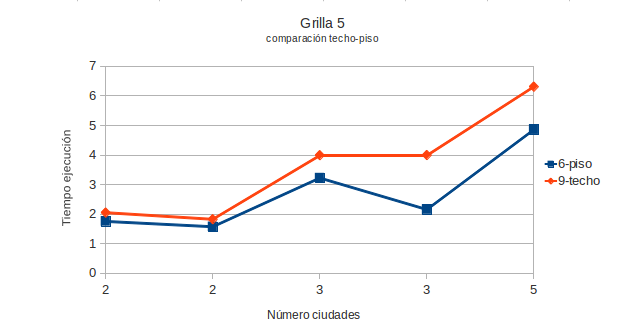
\includegraphics[scale=0.4]{./grilla5ceilfloor.png}
 % grilla5ceilfloor.png: 624x328 pixel, 72dpi, 22.01x11.57 cm, bb=0 0 624 328
 \caption{Comparación mejores techo y piso}
 \label{fig:grid5ceilfloor}
 \end{minipage}
\end{figure}









\end{document}